%*************************************************************************
%* Copyright © 2012-2016 Vincent Prat & Simon Nicolas
%*
%* This document is free; you can redistribute it and/or modify
%* it under the terms of the GNU General Public License as published by
%* the Free Software Foundation; either version 3 of the License, or
%* (at your option) any later version.
%*
%* This document is distributed in the hope that it will be useful,
%* but WITHOUT ANY WARRANTY; without even the implied warranty of
%* MERCHANTABILITY or FITNESS FOR A PARTICULAR PURPOSE. See the
%* GNU General Public License for more details.
%*
%* You should have received a copy of the GNU General Public License along
%* with this document; if not, write to the Free Software Foundation, Inc.,
%* 51 Franklin Street, Fifth Floor, Boston, MA 02110-1301 USA.
%*************************************************************************

\documentclass[a4paper,12pt]{article}

\usepackage[utf8]{inputenc}
\usepackage{lmodern}
\usepackage{graphicx}
\usepackage{hyperref}
\usepackage{xspace}
\usepackage{html}

\graphicspath{{images/}}

\newcommand*{\GMA}{GM-Assistant\xspace}
\newcommand*{\interfaceitem}[1]{\texttt{#1}}
\newcommand*{\versionnumber}{1.2\xspace}

\title{\GMA \versionnumber: user guide}
\author{Simon Nicolas \and Vincent Prat}
\date{5th January 2015}

\begin{document}

\maketitle

\latex{\tableofcontents}

\section{Introduction}

A role-playing game is a rich and complex alchemy.
The players have to be involved and the game master (GM) must perfectly master the rules and the scenario, remember previous events, anticipate the future, and improvise the present, following players' actions and choices.
If during the game the GM has to look about a non-player character (NPC) something specific in the rules, music or sound effects on the computer, images in a folder, then the game slows down, the emulsion fails, and the players lose their focus.
Do not deny it : role players are easily distracted.

The solution is \GMA.
\GMA (for \emph{Game Master Assistant}) is software designed to assist the GM. Its purpose is to simplify the GM’s life during the game by giving an easy access to relevant information and tools needed.

The purpose of this user guide is to help the user (you, the GM) to get used to the software. A menu bar, presented in Section ~\ref{menu}, and six modules, detailed in Section~\ref{sec:modules}, compose the main window. The sofware includes additionnal tools presented in Section~\ref{sec:tools}.
Finally, you can find the list of keyboard shortcuts in Appendix~\ref{sec:shortcuts}. 

\section{Menus}
\label{menu}

The menu bar of \GMA is quite similar to the one found in most applications.
Let us detail them one by one.
\subsection{Game}
\label{sec:game}

This menu gathers all the commands needed to manage your saves:
\begin{description}
    \item[\interfaceitem{New}:]{Creates a new scenario file}
    \item[\interfaceitem{Reload}:]{Returns the open scenario file to the state of its last save}
    \item[\interfaceitem{Load}:]{Loads a scenario file}
    \item[\interfaceitem{Recent}:]{Offers the list of recently opened scenario files}
    \item[\interfaceitem{Save}:]{Saves the open scenario file}
    \item[\interfaceitem{Save as}:]{Saves the open scenario file as a new file}
    \item[\interfaceitem{Metadata}:]{Displays a window with data about the scenario, such as the title, the author, the creation date, a short abstract, the list of players and the date of the game}
    \item[\interfaceitem{Quit}:]{Closes the scenario file and the application}
\end{description}

\latex{\paragraph{The save file}}

The save file \texttt{.gms} created is a file with everything included -- all the information and the auxiliary files (music, sound effects and images) -- so you can move it to another computer and use it without any trouble.

\subsection{Edit}
\label{sec:edit}

This menu is here to help the user in creating the scenario file. Two actions are currently available:
\begin{description}
    \item[\interfaceitem{Undo}:]{Cancels the last modification}
    \item[\interfaceitem{Redo}:]{Restores the last modification}
\end{description}

\subsection{View}
\label{sec:view}

This menu is here to choose the display options.
\begin{description}
    \item[\interfaceitem{Interface}:]{Opens a list of predefined setups of modules (see Section \ref{sec:modules} for details on modules)
        \begin{description}
            \item[\interfaceitem{Full}:]{All 6 modules}
            \item[\interfaceitem{Simple}:]{\interfaceitem{Plot}, \interfaceitem{Music} and \interfaceitem{Sound effects}}
            \item[\interfaceitem{Music}:]{\interfaceitem{Music} and \interfaceitem{Sound effects}}
            \item[\interfaceitem{Creation}:]{\interfaceitem{Plot}, \interfaceitem{Characters} and \interfaceitem{Notes}}
            \item[\interfaceitem{No sound}:]{\interfaceitem{Plot}, \interfaceitem{History}, \interfaceitem{Characters} and \interfaceitem{Notes}}
        \end{description}
    }
\item[\interfaceitem{Language}:]{Opens the list of languages available. At the moment, English and French are supported.}
\end{description}

\subsection{Tools}
\label{sec:menu_tools}

The menu gathers secondary tools. All the details are available in Section~\ref{sec:tools}. In the current version this menu includes:
\begin{description}
    \item[\interfaceitem{Dice simulator}:]{to launch dice}
    \item[\interfaceitem{Combat manager}:]{to structure the progress of combats}
\end{description}

\subsection{Help}
\label{sec:help}

Opens general information on the software and its license.

\section{Modules}
\label{sec:modules}

As already mentioned, there are 6 independent blocs we call modules, each dedicated to one functionality. Several modules are ``trees'', in which you can organize information. Possibilities given by these trees and items inside are explained in Section~\ref{item}.
The list of modules includes:
\begin{description}
    \item[\interfaceitem{Plot}:]{The plot tree is designed to show in an ordered manner the important events of the scenario with no limit in sub-levels}
    \item[\interfaceitem{History}:]{Same as the plot tree, designed for important events taken from previous games}
    \item[\interfaceitem{Notes}:]{Simple notepad to take notes during the scenario}
    \item[\interfaceitem{Characters}:]{A table designed to display the characters (players or NPC) with their important statistics}
    \item[\interfaceitem{Music}:]{A simple music player}
    \item[\interfaceitem{Sound effects}:]{A simple music player designed for short sounds like gunshots, bell ringing, screams, etc.}
\end{description}
All these modules are available in the main interface of the software.
\begin{figure}[ht]
    \centerline{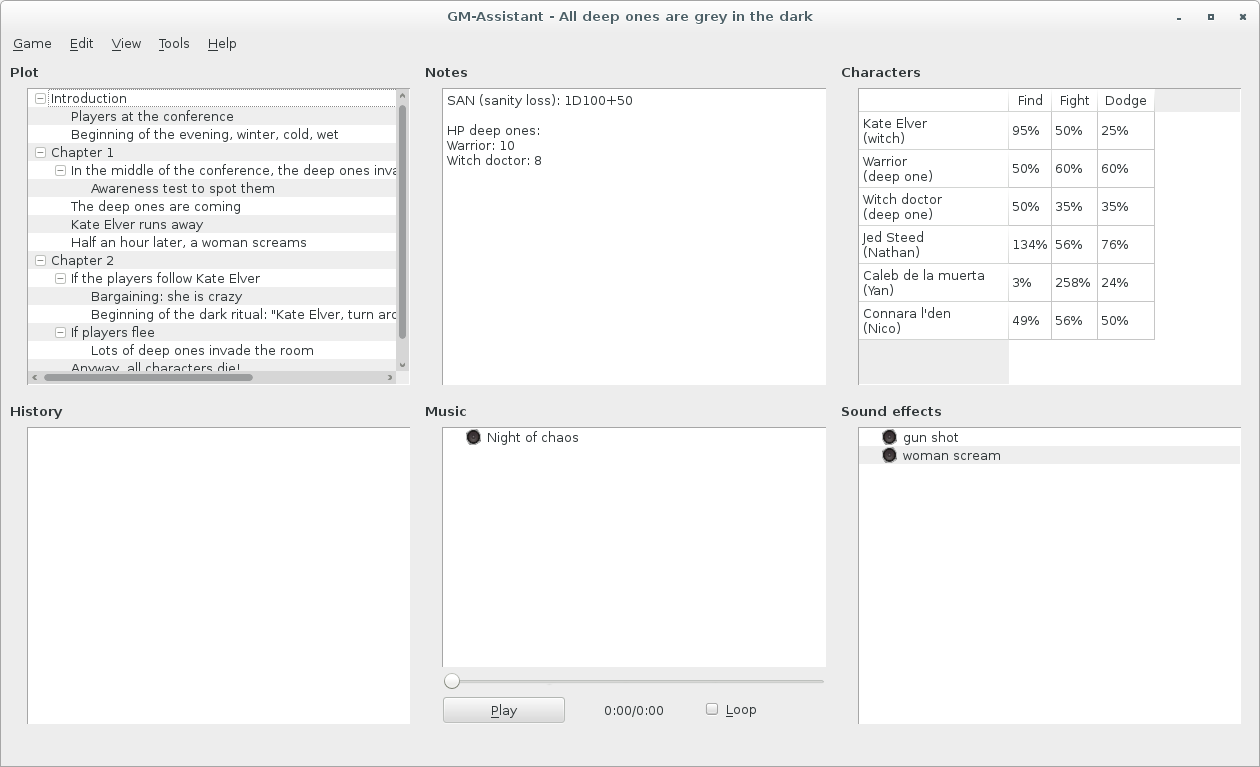
\includegraphics[width=\textwidth]{full_scenario}}
    \caption{Main window}
    \label{fig:interface}
\end{figure}

\subsection{Items}
\label{item}

Items are the basis of \GMA, since they are found almost everywhere in the software. It is therefore important to explain their specifics in the modules themselves.
The definition of an item is the smallest element of something.
In our case, an item is a line, an object of a module in the software.
Each item has a state, giving a quick look of the failure or success of certain key events of the plot.
The four states are: \interfaceitem{None}, \interfaceitem{In progress}, \interfaceitem{Failed} and \interfaceitem{Succeeded}.
An item can also carry additional contents, following its type: \interfaceitem{Basic} (nothing more), \interfaceitem{Audio} (sounds or music) ou \interfaceitem{Image} (any kind of image).
The modules using items are: \interfaceitem{Plot}, \interfaceitem{History}, \interfaceitem{Music} and \interfaceitem{Sound effects}.
Right click on an item and the item menu appears. In this menu are the four states and three actions: \interfaceitem{Add}, \interfaceitem{Delete}, \interfaceitem{Edit}.
If the type of the item is \interfaceitem{Audio} or \interfaceitem{Image}, two more actions are available: one to play the file (or show it) and one to export the file.
For \interfaceitem{Audio} files, the action \interfaceitem{Play} only shows in modules \interfaceitem{Music} and \interfaceitem{Sound effects}.

The action \interfaceitem{Add} gives access to the item creation window.
\begin{figure}[ht]
    \centerline{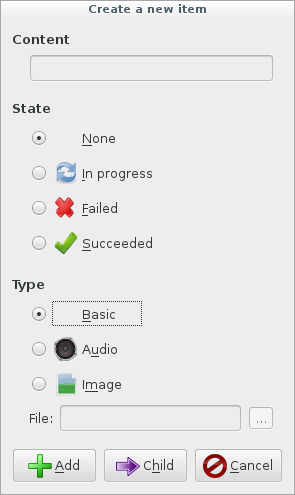
\includegraphics[width=0.4\textwidth]{add_item}}
    \caption{Item creation window}
    \label{fig:ajout}
\end{figure}
This window can also be accessed by right clicking in the empty part of the module or pressing the \interfaceitem{Insert} key on the keyboard.
The window is organized as follows:
\begin{itemize}
    \item In \interfaceitem{Content} is are the information/description of the event;
    \item In \interfaceitem{State} is set the default state of the item;
    \item In \interfaceitem{Type} is chosen the type of the item: \interfaceitem{Basic} (just text), \interfaceitem{Music}, or \interfaceitem{Image}. The last two unlock the ``File'' entry to choose the file associated to the item;
    \item The \interfaceitem{Add} button adds the item after the selected item at the same level of the hierarchy;
    \item The \interfaceitem{Child} button adds the item after and as a child of the selected item;
    \item The \interfaceitem{Cancel} button cancels the creation.
\end{itemize}
It is important to see the difference between \interfaceitem{Add} and \interfaceitem{Child} buttons. This is how the tree is organized.
Note: items can be moved by drag-and-drop.

\subsection{Plot Tree}
\label{sec:plot}

The plot tree is, almost every time, the core of \GMA., where the detailed and structured plot elements are gathered, so no important element is forgotten.
Figure ~\ref{arbre_scenar} shows an example of what is possible.
\begin{figure}[ht]
    \centerline{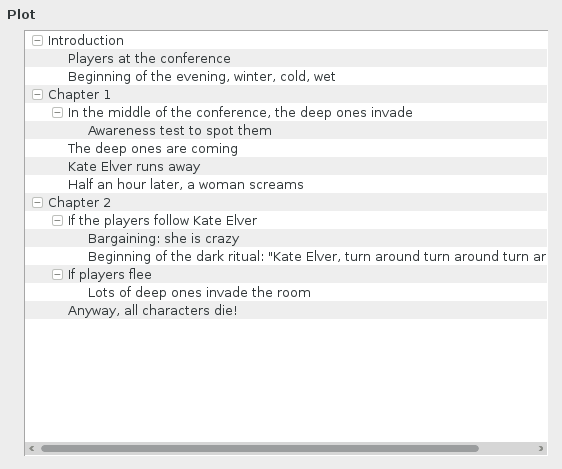
\includegraphics[width=0.7\textwidth]{sample_scenario}}
    \caption{Example of scenario}
    \label{arbre_scenar}
\end{figure}

Each line is an item and one just needs to follow the item creation procedure described in Section~\ref{item} to organize the scenario.
Do not forget that the state of an item can be modified during the game to keep track of the progression of players in the plot. It can be useful if the scenario goes across several game sessions.

\subsection{History}
\label{sec:history}

The History tree is meant to keep track of important events that occurred in previous sessions, such as important encounters, a promise, a lie, etc.
It is also possible to write down some elements of the players' past.
In this way all these facts are quickly available to the GM.
Technically, the History behavior is the same as the plot tree.

\subsection{Notes}
\label{sec:notes}

The Notes module is a simple text editor. To write text, just left-click somewhere in the module to write any useful items to remember.
For instance: “Mike insulted the museum director.”
This module can also be used during the preparation of the scenario to add details to complex elements such as events, history or characters.

\subsection{Characters}
\label{sec:char}

The Characters module is designed to show the list of the protagonists and the relevant information needed about them during the game.
These data are called “properties” and can be either text or numbers. In the module, characters are lines and properties are columns.
As for the tree modules, building the table is done by right-clicking on it. It shows a popup menu containing all the available actions. When the module is empty, the submenus \interfaceitem{Character} and \interfaceitem{Property} allow you to add a character or a property through the \interfaceitem{Add} action. A window pops up to enter the name. In the case of a character, a second entry is available to add a short detail such as the name of the character’s player.
Once there is at least one character and one property, editable cells appear to receive the values of the properties. Right-click on a cell to open the same popup menu as before, which will now show the possibility to delete and edit the character or property. 
Please note that once a character or a property is created, a right click on the related upper band  (horizontal for properties, vertical for characters) will directly open the corresponding submenu.


\subsection{Music}
\label{sec:music}

The Music module is a simple music player for background music or continuous sounds (such as rain or wind). Please note it is only possible to play one sound at a time.
The module is in two parts: a tree similar to \interfaceitem{Plot} and \interfaceitem{History} to organize the music and the player itself, made up of:

\begin{itemize}
    \item a scroll bar and a counter showing the position in the music file,
    \item a button to control the playback,
    \item a checkbox to toggle the loop playback option.
\end{itemize}
When there is no music playing, \interfaceitem{Play} is written on the button. Push it to play the selected file, and the button will turn to \interfaceitem{Pause}. Click once again to pause, and the button will turn to \interfaceitem{Resume}.

\subsection{Sound effects}
\label{sec:fx}

The Sound effects module is an even simpler music player, designed to play very short sounds such as gunshot, scream, etc. Unlike the Music module, there is only a tree; to play a sound, just double-click on a sound item.
A sound can be played while music is playing in the Music module. But if a sound is played before another one is finished, the second one will replace the first one.
There is no way to stop a sound before its natural end.


\section{Tools}
\label{sec:tools}
Like modules, tools are meant to help the GM during games, but unlike them, they are not used to store data. The two tools available in the current version are a dice simulator (see Section~\ref{sec:dice}) and a combat manager (see Section~\ref{sec:combat}).

\subsection{Dice simulator}
\label{sec:dice}

The dice simulator is a tool allowing the user to simulate directly in the software the random result of virtual dice. You will have all you need if you forget your dice or if you want to roll more dice than you have. To use it, select this option in the \interfaceitem{Tools} menu. A window similar to figure~\ref{simulateur_des} will open.
\begin{figure}[ht]
    \centerline{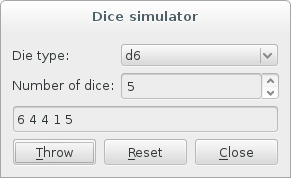
\includegraphics[width=0.4\textwidth]{dice_simulator}}
    \caption{Dice simulator}
    \label{simulateur_des}
\end{figure}

This window allow the user to choose among these elements:
\begin{description}
    \item[Die type:]{The number of faces of each die. If you are unfamiliar with concepts in role-playing games, d$n$ is a die with $n$ faces.}
    \item[Number of dice:]{The number of dice you will roll, maximum 10.}
\end{description}

\subsection{Combat manager}
\label{sec:combat}

In all role-playing games, fights are quite hard to manage. Indeed, the GM has to remember the order each character plays in, count the hit points and wounds of each protagonist, etc. To help the GM in this sometimes-hard task, \GMA offers the combat manager.

As with the dice simulator, clicking the appropriate option in the \interfaceitem{Tools} menu opens the combat manager. Its use is in two steps: the selection of the different protagonists and the fight itself.

\subsubsection{Selection of participants}
A window similar to Figure~\ref{gestion_combat_choix} appears. The list of protagonists on the left side is automatically generated from the \interfaceitem{Characters} module. You have to select each protagonist involved in the fight to add it to the right side by clicking on \interfaceitem{Add}. If you make a mistake, you can remove a protagonist by clicking on it on the right side and then on the \interfaceitem{Remove} button.
\begin{figure}[ht]
    \centerline{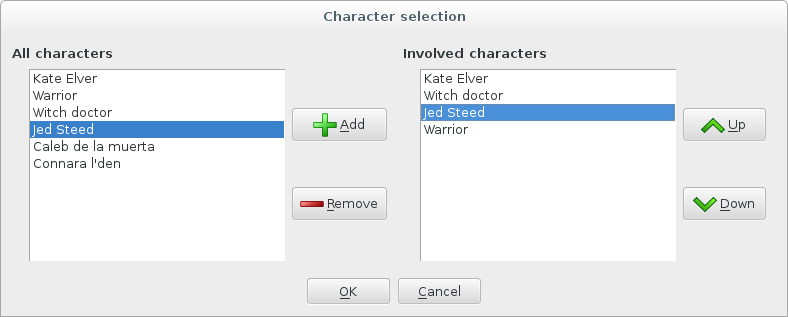
\includegraphics[width=1\textwidth]{combat_preparation}}
    \caption{Combat manager: selection of protagonists}
    \label{gestion_combat_choix}
\end{figure}

The order of the actors on the right side is the order in which they will act. Use the \interfaceitem{Up} and \interfaceitem{Down} buttons to order the list, which can be changed at any time during the fight. When you are ready, click \interfaceitem{OK} to move to the next step.

\subsubsection{Fight}

Now appears the Combat manager itself, as shown in Figure~\ref{gestion_combat_fight}.
\begin{figure}[ht]
    \centerline{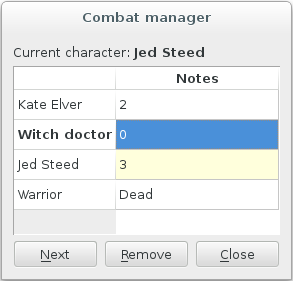
\includegraphics[width=0.4\textwidth]{combat_fight}}
    \caption{Combat manager: fight}
    \label{gestion_combat_fight}
\end{figure}
Again, the list of the different protagonists and column notes appears.
It can be useful to note the wounds, hit points, or anything else you want to keep in mind. To use it, double click on the cell or press \interfaceitem{F2} when selected. Every turn, the name of the current protagonist is displayed. The \interfaceitem{Note} cell of this character appears in yellow. When the protagonist has finished its move, click on \interfaceitem{Next} button to go to the next protagonist.
In case one protagonist has to quit the fight (death, run away) it can be removed by clicking on \interfaceitem{Delete} after selecting it. If at some point a protagonist wants to delay its action or if you have made a mistake, it is possible to move by dragging and dropping to the right place. The next protagonist automatically becomes active.
When the fight is over, click on \interfaceitem{Close}.

\section{Conclusion}\label{conclusions}
\GMA is software built by role-players for role-players. We encourage you to try it to see if it suits you. If for any reason you are not satisfied with it, please note that we do our best. In any case, feel free to participate in the enhancement of this software by:
	\begin{itemize}
    \item Using the software, giving us your feedback, and making bug reports;
    \item Making this software known;
    \item Proposing new functionality;
    \item Reading and helping to write the guide;
    \item Translating the software and the user guide;
    \item Maintaining the website 
 \url{http://gmassistant.free.fr};
    \item Joining the dev team.
\end{itemize}

Contact us at \url{gmassistant@free.fr}.
If you have a Github account, you can also follow the project, inspect the code, and report bugs on the project page: \url{http://github.com/ViviCoder/GM-Assistant}.
Finally, if you want to be up-to-date about what concerns GM-Assistant, you can subscribe to the RSS: http://gmassistant.free.fr/feed. \url{http://gmassistant.free.fr/feed}.

\appendix

\section{List of keyboard shortcuts}
\label{sec:shortcuts}

\subsection{Menus}

\begin{description}
    \item[\interfaceitem{Ctrl+B}:]{Combat manager}
    \item[\interfaceitem{Ctrl+D}:]{Dice simulator}
    \item[\interfaceitem{Ctrl+M}:]{Metadata}
    \item[\interfaceitem{Ctrl+N}:]{New game}
    \item[\interfaceitem{Ctrl+O}:]{Load}
    \item[\interfaceitem{Ctrl+Q}:]{Quit}
    \item[\interfaceitem{Ctrl+R}:]{Reload}
    \item[\interfaceitem{Ctrl+S}:]{Save}
    \item[\interfaceitem{Ctrl+Shift+S}:]{Save as}
    \item[\interfaceitem{Ctrl+Z}:]{Undo}
    \item[\interfaceitem{Ctrl+Shift+Z}:]{Redo}
    \item[\interfaceitem{F1}:]{About}
    \item[\interfaceitem{F5}:]{Full}
    \item[\interfaceitem{F6}:]{Simple}
    \item[\interfaceitem{F7}:]{Music}
    \item[\interfaceitem{F8}:]{Creation}
    \item[\interfaceitem{F9}:]{No sound}
\end{description}

\subsection{Trees}

\begin{description}
    \item[\interfaceitem{Space}:]{Play (music or sound effects) or Show (Picture)}
    \item[\interfaceitem{Ins}:]{Add}
    \item[\interfaceitem{Del}:]{Delete}
    \item[\interfaceitem{+}:]{Unfold}
    \item[\interfaceitem{-}:]{Fold}
    \item[\interfaceitem{F2}:]{Simple edition}
    \item[\interfaceitem{Ctrl+F2}:]{Complete edition}
    \item[\interfaceitem{Ctrl+F5}:]{State \interfaceitem{None}}
    \item[\interfaceitem{Ctrl+F6}:]{State \interfaceitem{In progress}}
    \item[\interfaceitem{Ctrl+F7}:]{State \interfaceitem{Failed}}
    \item[\interfaceitem{Ctrl+F8}:]{State \interfaceitem{Succeeded}}
\end{description}

\subsection{Table}

\begin{description}
    \item[\interfaceitem{Ctrl+Ins}:]{Add a property}
    \item[\interfaceitem{Ctrl+Shift+Ins}:]{Add a character}
    \item[\interfaceitem{Del}:]{Delete a cell}
    \item[\interfaceitem{Ctrl+Del}:]{Delete a property}
    \item[\interfaceitem{Ctrl+Shift+Del}:]{Delete a character}
    \item[\interfaceitem{F2}:]{Edit a cell}
    \item[\interfaceitem{Ctrl+F2}:]{Edit a property}
    \item[\interfaceitem{Ctrl+Shift+F2}:]{Edit a character}
\end{description}

\end{document}
